\chapter{Cloudbreak}\label{chap_cloudbreak_impl}

In the previous chapter, we described and formalized a general strategy for building SV detection algorithms in MapReduce and Hadoop. In this chapter, we describe an software package, Cloudbreak, that we have developed using this algorithmic framework. To build Cloudbreak, we implemented the infrastructure necessary to support the algorithmic framework we described in Section~\ref{section_general_algo}, and also provided implementations of the three application-specific functions we described there. Here we will describe this implementation, as well as our choices for the three user-defined functions we specified in the framework definition, and additional functionality we developed to genotype calls and to facilitate the deployment of Cloudbreak on public cloud platforms including Amazon's EC2. In Chapter~\ref{chap_cloudbreak_eval}, we will provide an evaluation of the algorithm's accuracy and performance characteristics.

\section{Variant types detected}

Cloudbreak is our implementation of a detection algorithm for genomic deletions (40bp-25,000bp) and small insertions based on examining the insert sizes of paired end mappings. We chose this application because small deletions in the range of 50bp to 150bp are particularly difficult to detect using many existing SV algorithms~\cite{Alkan:2011p547,Mills:2011fi}. This is because most read-pair based algorithms use a hard cutoff based on the variance of the fragment size distribution to select discordant read pairs, as described in Section~\ref{section_read_pair}. By taking advantage of many compute cores using MapReduce, we can design an algorithm that considers all of available data (both concordant and discordant read pairs) in a generative statistical framework, as we will describe in Section~\ref{section_user_defined_functions}.

\section{Framework infrastructure}

In addition to the specific algorithm for detecting deletions and insertions (which take the form of implementations of the user-defined functions we described in the previous chapter), the Cloudbreak package also contains the infrastructure necessary to implement the three MapReduce jobs defined in our MapReduce algorithmic framework. Providing a fully featured, multi-job Hadoop application requires several implementation decisions:

\begin{itemize}
\item \textbf{Programming language and method of interacting with Hadoop.} Hadoop applications can be developed in several ways. A native application is written in Java and directly uses the Hadoop application programming interface (API) to start jobs, implement Map and Reduce functions, and set advanced Hadoop configurations. Alternatively, applications can be developed in any language using the Hadoop \emph{streaming} interface, as long as the input to and output from all map and reduce tasks is textual and certain conventions are followed with respect to data format. Finally, for C/C++ applications, the Hadoop \emph{pipes} interface can be used to marshal input and output data from tasks. Each method has its own advantages and disadvantages. Native applications constrain the developer to Java but enjoy the best performance when the jobs are data intensive rather than CPU bound~\cite{Ding:2011:MCM:2103380.2103444}. Streaming applications allow greater programming language flexibility but make it somewhat more difficult to organize complex applications and take advantage of advanced Hadoop features. Pipes, meanwhile, allow for maximum performance for CPU intensive applications. We opted to develop Cloudbreak as a native application to take advantage of the tight integration with the Hadoop API improved I/O performance on data intensive portions of the workflow. For the \textsc{Align Reads} job, which executes existing short-read alignment tools, a mapper class written in Java invokes the external tools using the system runtime environment.

\item \textbf{File formats and compression.} Hadoop applications usually store their data in HDFS in text format or in sequence files, a binary format that allows numeric or complex data types to be stored in a key-value pair structure easily accessed by Hadoop. In addition, varying levels of compression can be used, although only certain compression types allow Hadoop to automatically split large files by HDFS blocks for processing by different map tasks, which is a key consideration for building fully parallelized applications. Cloudbreak uses sequence files for input and intermediate files, although for alignments the values are stored as text strings containing full records in the Sequence Alignment Map (SAM) format~\cite{Li:2009vz}, to allow for easy exports of data. For compression we use the Snappy~\cite{snappy} compressor/decompressor (codec), a compression scheme developed at Google which aims for reasonable file size reduction with very fast compression and decompression speeds. This makes it ideal for data-intensive Hadoop applications. Given that the output data from the \textsc{Align Reads} job is alignment records, a future implementation goal is to switch to using Hadoop-BAM~\cite{Niemenmaa:2012hu}, a library for storing SAM/BAM records efficiently in HDFS; Hadoop-BAM did not posses necessary functionality at the time of Cloudbreak's initial implementation and so we proceeded with a text-based representation of alignment records.

\item \textbf{Distribution of auxiliary files.} In some cases all tasks require access to large input files, such as genome reference indices for alignment, or genome annotation files. Hadoop offers a \emph{distributed cache} service, which places copies of the files on each node that will host tasks for the job so that they will not all need to copy the files over the network. Cloudbreak makes use of the distributed cache to distribute index and annotation files, as well as the alignment executables for the \textsc{Align Reads} job.
\end{itemize}

Our implementation of the \textsc{Align Reads} job contains wrappers to execute the aligners BWA \cite{Li:2009p836}, GEM \cite{MarcoSola:2012hm}, Novoalign \cite{novoalign}, RazerS 3 \cite{Weese:2012by}, mrFAST \cite{Alkan:2009cr}, and Bowtie 2 \cite{Langmead:2012jh}. This job can also be skipped in favor of importing a pre-aligned BAM file directly into HDFS. The code is structured in such a way that to add a new aligner, developers would simply create a class that finds the necessary index files in the distributed cache and determines the proper command line parameters for aligner execution, and parses the aligner output if it is in a non-standard format.

Cloudbreak can be executed on any Hadoop cluster; Hadoop abstracts away the details of cluster configuration, making distributed applications portable. We deployed Cloudbreak on an internal 56-node cluster running the Cloudera CDH3 Hadoop distribution, version 0.20.2-cdh3u4. In addition, Cloudbreak can create and operate on Hadoop clusters located in commercial and private compute clouds (see Section~\ref{section_cloud_whirr}).

The source code and user manual for Cloudbreak are publicly available at \url{https://github.com/cwhelan/cloudbreak}. We hope that by publishing under an open-source license, we will facilitate the adoption of our Cloudbreak implementation, as well as provide a base from which other computational researchers can develop their own SV detection algorithms for Hadoop.

\section{Implementation of a MapReduce SV Algorithm}\label{section_user_defined_functions}

In Section~\ref{section_general_algo}, we described three user-defined functions that can be implemented to create an SV detection application in our MapReduce framework. These functions were named \textsc{Loci}, $\Phi$, and \textsc{PostProcess}. These functions map aligned read pairs to locations on the genome to which they are relevant, compute a set of local features for each genomic location based on the relevant read pairs, and call variants based on the features computed for neighboring genomic locations. Cloudbreak contains implementations of these functions that combine to allow it to detect deletions (of size 40bp-25,000bp) and insertions. A detailed description of each of these implementations appears below, and an illustration of each phase of the Cloudbreak algorithm working on a simple example in MapReduce is shown in Figure \ref{cloudbreak_example}.

\begin{figure}
\centering
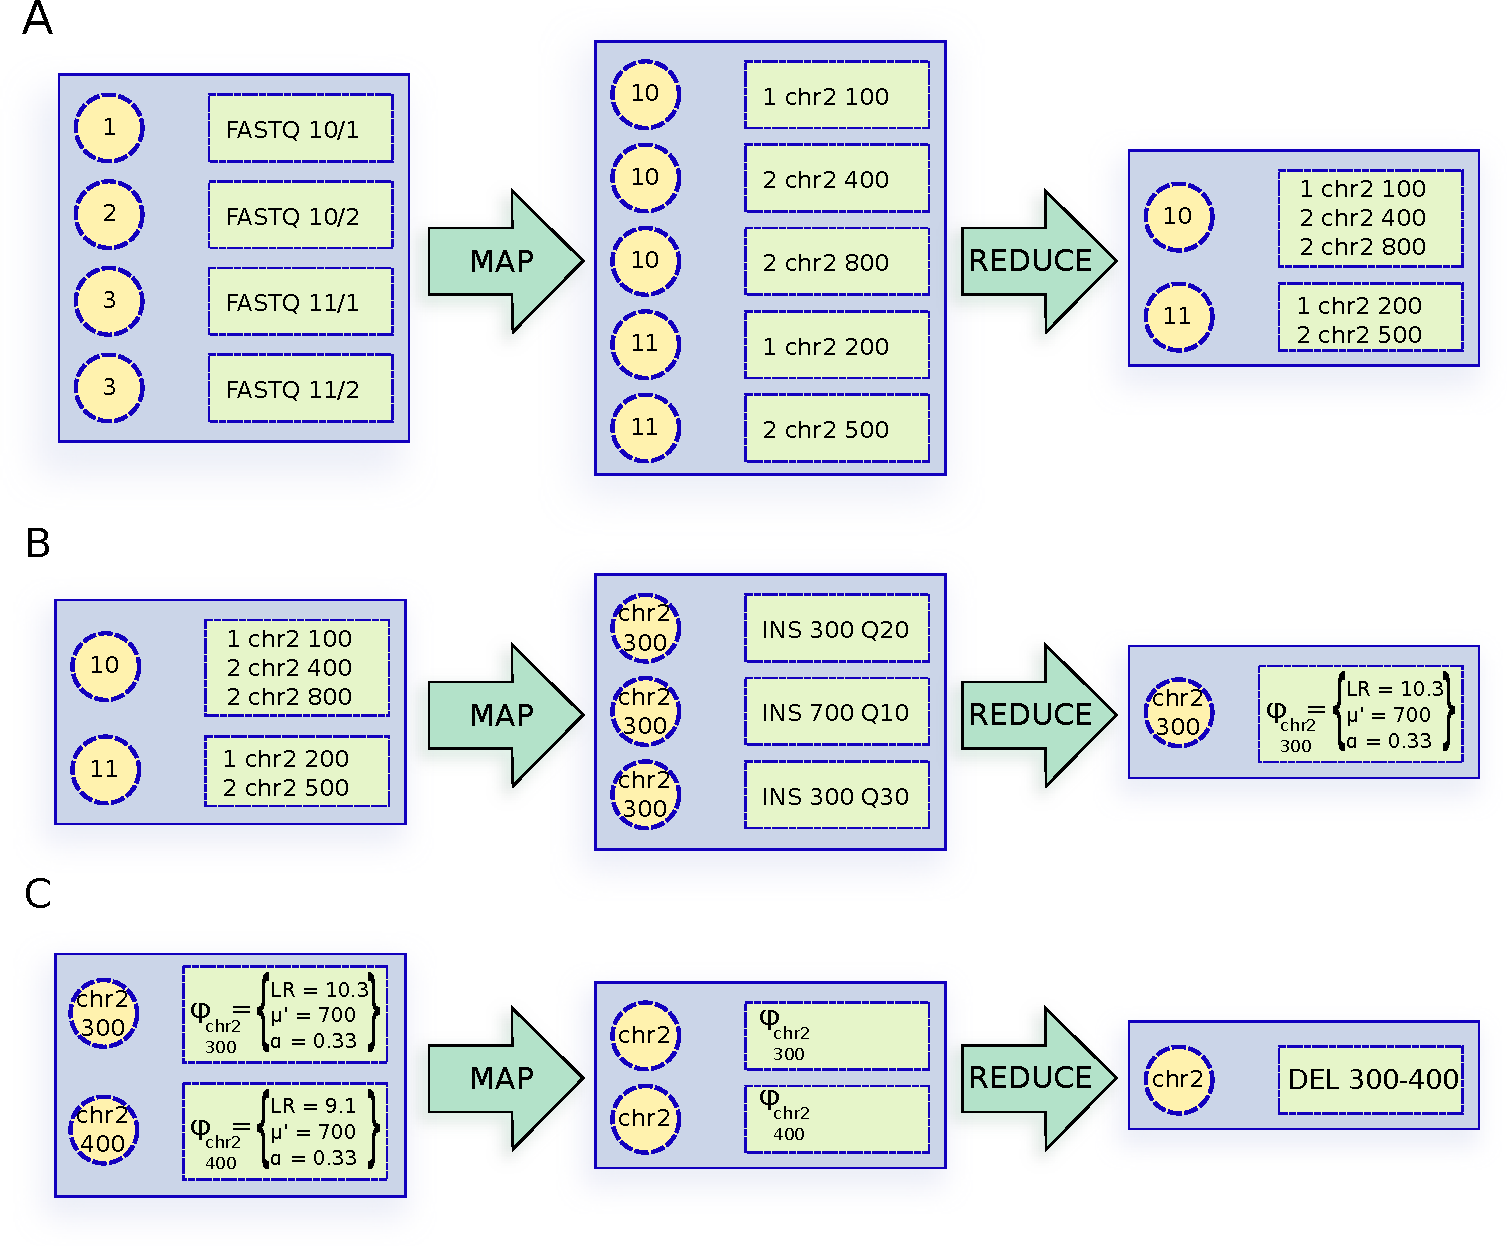
\includegraphics[width=.9\textwidth]{/users/cwhelan/Documents/svpipeline/figures/cloudbreak_mapred_diagram.pdf}
\caption[An Example of the Cloudbreak deletion and insertion detection algorithm running in MapReduce.]{An Example of the Cloudbreak deletion and insertion detection algorithm running in MapReduce. A) In the first MapReduce job, mappers scan input reads in FASTQ format and execute an alignment program in either paired-end or single-ended mode to generate read mappings. Reducers gather all alignments for both reads in each pair. B) In the second MapReduce job, mappers first emit information about each read pair (in this case the insert size and quality) under keys indicating the genomic location spanned by that pair. Only one genomic location is diagrammed here for simplicity. Reducers then compute features for each location on the genome by fitting a GMM to the distribution of spanning insert sizes. C) Mappers group all emitted features by their chromosome, and reducers find contiguous blocks of features that indicate the presence of a variant.}
\label{cloudbreak_example}
\end{figure}

\begin{description}
\item[\sc{Loci}] Because we are detecting deletions and short insertions, we map ReadPairInfos from each possible alignment to the genomic locations overlapped by the implied internal insert between the reads. For efficiency, we define a maximum detectable deletion size of 25,000bp, and therefore alignment pairs in which the ends are more than 25kb apart, or in the incorrect orientation, map to no genomic locations. In addition, if there are multiple possible mappings for each read in the input set, we optimize this step by assuming that if there exists a concordant mapping for a read pair, defined as a mapping pair in which the two alignments are in the proper orientation and with an insert size within three standard deviations of the expected library insert size, it is likely to be correct and therefore we do not consider any discordant alignments of the pair.

\item[$\Phi$] To compute features for each genomic location, we follow the mixture of distributions approach (see Section~\ref{section_mixture_of_distributions}) first described by Lee et al.~\cite{Lee:2009da}, who observed that if all mappings are correct, the insert sizes implied by mappings which span a given genomic location should follow a Gaussian mixture model (GMM) whose parameters depend on whether a deletion or insertion is present at that locus. Figure~\ref{insert_size_mixes} shows several examples of the mixtures observed for various types of variants. If there is no indel, the insert sizes implied by spanning alignment pairs should follow the distribution of actual fragment sizes in the sample, which is typically modeled as normally distributed with mean $\mu$ and standard deviation $\sigma$. If there is a homozygous deletion or insertion of length $l$ at the location, $\mu$ should be shifted to $\mu + l$, while $\sigma$ will remain constant. Finally, in the case of a heterozygous event, the distribution of insert sizes will follow a mixture of two normal distributions, one with mean $\mu$, and the other with mean $\mu + l$, both with an unchanged standard deviation of $\sigma$, and mixing parameter $\alpha$ that describes the relative weights of the two components. The features generated for each location $l$ include the log-likelihood ratio of the filtered observed data points under the fit GMM to their likelihood under the distribution $N(\mu,\sigma)$, the final value of the mixing parameter $\alpha$, and $\mu'$, the estimated mean of the second GMM component. 

The choice of a mixture of distributions model has several benefits. Firstly, it is a generative model for the entire data set, including concordant and discordant read pairs. This removes the need to set hard thresholds that define discordant read pairs, and allows the detection of smaller variants given a tight enough insert size distribution. Second, the parameters that are estimated can be used to refine and classify predictions. For example, the mixing parameter $\alpha$ can be used to genotype variants, as we will describe in Section~\ref{section_genotyping}. In addition, the estimated $\mu'$ parameter gives a prediction for how many genomic locations the variant might cover, which we leverage in the \textsc{PostProcess} function described below to integrate local features into variant calls.

To implement our model, at each genomic location we fit the parameters of the GMM using the Expectation-Maximization algorithm. Let $Y = y_{1,2, \ldots m}$ be the observed insert sizes at each location after filtering, and say the library has mean fragment size $\mu$ with standard deviation $\sigma$. Because the mean and standard deviation of the fragment sizes are selected by the experimenter and therefore known \emph{a priori} (or at least easily estimated based on a sample of alignments), we only need to estimate the mean of the second component at each locus, and the mixing parameter $\alpha$. Therefore, we initialize the two components to have means $\mu$ and $\bar{Y}$, set the standard deviation of both components to $\sigma$, and set $\alpha = .5$. In the E step, we compute for each $y_i$ and GMM component $j$ the value $\gamma_{i,j}$, which is the normalized likelihood that $y_i$ was drawn from component $j$. We also compute $n_j = \sum_i{\gamma_{i,j}}$, the relative contributions of the data points to each of the two distributions. In the M step, we update $\alpha$ to be $n_2 - \left|Y\right|$, and set the mean of the second component to be $\frac{\sum_m{\gamma_{m,2}y_m}}{n_2}$. We treat the variance as fixed and do not update it, since under our assumptions the standard deviation of each component should always be $\sigma$. We repeat the E and M steps until convergence, or until a maximum number of steps has been taken. Prior to fitting the GMM at each location, we attempt to filter out incorrect mappings for that location using an outlier-detection based clustering scheme and an adaptive mapping quality cutoff; see Section~\ref{section_incorrect_and_ambiguous_mappings} for details.

\item[\sc{PostProcess}] The third MapReduce job is responsible for making SV calls based on the features defined above. We convert our features along each chromosome to insertion and deletion calls by first extracting contiguous genomic loci where the log-likelihood ratio of the two models is greater than a given threshold. To eliminate noise we apply a median filter with window size 5. We end regions when $\mu'$ changes by more than 60bp ($2\sigma$), and discard regions where the average value of $\mu'$ is less than $\mu$ or where the length of the region differs from $\mu'$ by more than $\mu$.
\end{description}

\begin{figure}
\centering
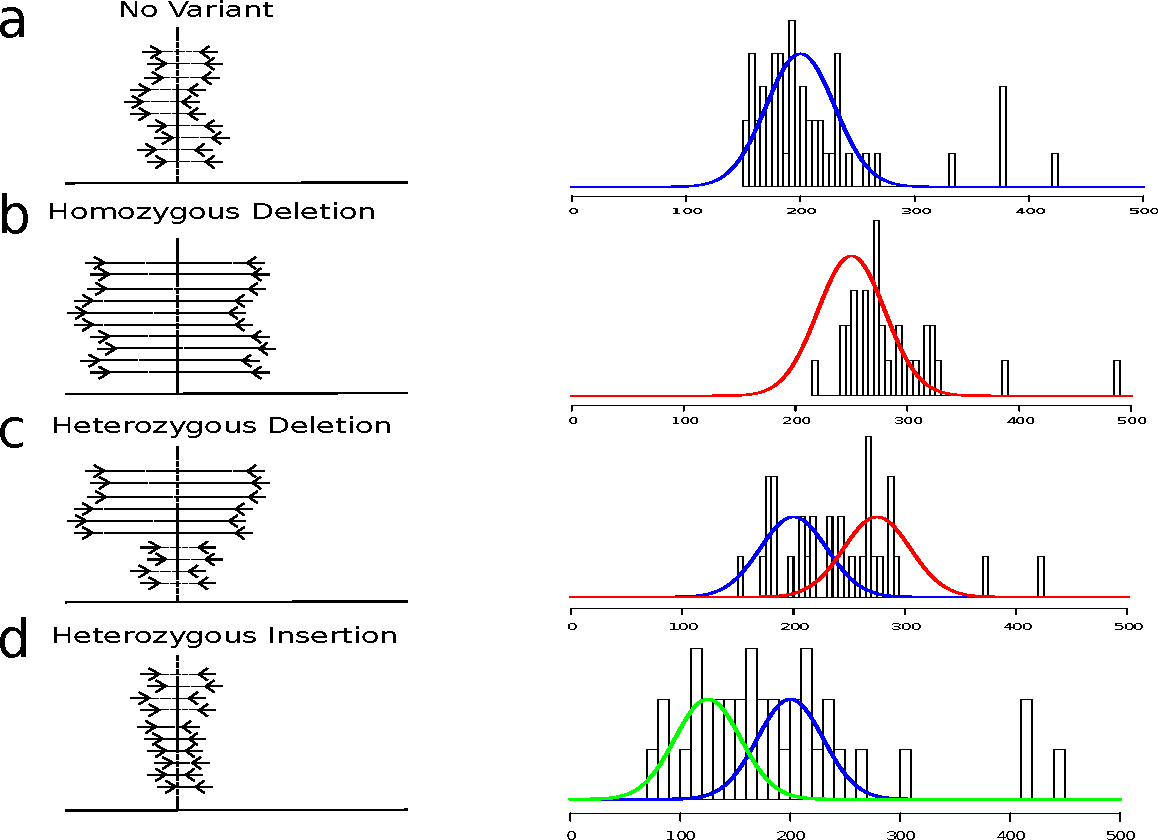
\includegraphics[width=.9\textwidth]{figures/insert_size_mixtures.pdf}
\caption[Illustration of insert size mixtures at individual genomic locations.]{Illustration of insert size mixtures at individual genomic locations. A) there is no variant present at the location indicated by the vertical line (left), so the mix of insert sizes (right) follows the expected distribution of the library centered at 200bp, with a small amount of noise coming from low-quality mappings. B) a homozygous deletion of 50bp at the location has shifted the distribution of observed insert sizes. C) A heterozygous deletion at the location causes a mixture of normal and long insert sizes to be detected. D) A heterozygous small insertion shifts a portion of the mixture to have lower insert sizes.}
\label{insert_size_mixes}
\end{figure}

\section{Filtering Incorrect and Ambiguous Mappings}\label{section_incorrect_and_ambiguous_mappings}

One of our goals in developing Cloudbreak was to see if the use of distributed computing in the MapReduce framework would allow us to develop an algorithm that could process multiple mappings for ambiguously mapped reads in a reasonable amount of time, especially because the size of data sets can grow very large if many possible mappings are kept for all ambiguous reads. Most SV detection tools that use multiple mappings attempt to identify the correct mapping for each ambiguously mapped pair; for example, GASVPro~\cite{Sindi:2012kk} uses an MCMC approach to sample from the distribution of possible mapping locations for each read, and VariationHunter~\cite{Hormozdiari:2009p284} attempts to assign mappings to reads through a combinatorial optimization approach. Cloudbreak, in contrast, attempts to solve this problem at the genomic location level by filtering mappings during the feature computation step.

To handle incorrect and ambiguous mappings, we assume that in general they will not form normally distributed clusters in the same way that correct mappings will, and therefore use an outlier detection technique to filter the observed insert sizes for each location. We sort the observed insert sizes and define as an outlier an observation whose $k$th nearest neighbor is more than $n\sigma$ distant, where $k = 3$ and $n = 5$. In addition, we rank all observations by the estimated probability that the mapping is correct and use an \emph{adaptive quality cutoff} to filter observations: we discard all observations where the estimated probability the mapping is correct is less than the score of the maximum quality observation minus a constant $c$. This allows the use of more uncertain mappings in repetitive regions of the genome while restricting the use of low-quality mappings in unique regions. Defining $\textsc{Mismatches}(a)$ to be the number of mismatches between a read and the reference genome in the alignment $a$, we approximate the probability $p^{k}_c$ of each end alignment being correct by:

\[ p^{k}_c(a^{k}_{m,i}) = \frac{\exp({-\textsc{Mismatches}(a^{k}_{m,i})/2)}}{\sum_j{\exp(-\textsc{Mismatches}(a^{k}_{m,j})/2)}} \]


By multiplying $p_c(a^{1}_{m,i})$ and $p_c(a^{2}_{m,i})$, we can approximate the likelihood that the pair is mapped correctly.

\section{Genotyping}\label{section_genotyping}

In theory, it should be possible to use the parameters of the fit GMM to infer the genotype of each predicted variant. Assuming that our pipeline is capturing all relevant read mappings near the locus of the variant, the genotype should be indicated by the estimated parameter $\alpha$, the mixing parameter that controls the weight of the two components in the GMM.  We set a simple cutoff on the average value of $\alpha$ for each prediction to call the predicted variant homozygous or heterozygous, and use the same cutoff for deletion and insertion predictions. Somewhat surprisingly, we observed on the cutoff point that distinguishes homozygous from heterozygous variants is significantly less than the expected .5; based on empirical observations on a simulated data set, we set the threshold to .35 (see Section~\ref{section_genotyping_eval} for more details).

\section{Running in the Cloud}\label{section_cloud_whirr}

In Section~\ref{section_seq_big_data}, we discussed the increasing recognition of the genomics community of the need for tools that ease the use of cloud computing resources~\cite{Schatz:2010js,Stein:2010gp}. This has spurred the development of a variety of applications and toolkits that use the APIs of Infrastructure as a Service (IaaS) providers, such as Amazon EC2, to allocate compute resources on public compute clouds. In this section, we will briefly review some of the existing cloud-enabled tools, including those that are based on traditional grid scheduling engines and those that enable Hadoop and MapReduce pipelines. Many of the latter take advantage of Amazon's Elastic MapReduce (EMR) service, an offering from Amazon specifically for creating and running Hadoop jobs that simplifies the creation and monitoring of clusters on EC2. We will then discuss how Cloudbreak enables the use of cloud computing in a provider-neutral way using the Apache Whirr library.

\subsection{Cloud-Enabled Genomics Tools}

Several groups have created general-purpose toolkits for creating, allocating, and managing cloud resources for biological data processing. For example, the CloudBioLinux project~\cite{Krampis:2012wo} provides virtual machine images for use in Amazon EC2 that are pre-configured with a wide range of open-source bioinformatics applications. Galaxy CloudMan~\cite{Afgan:2010fa} allows for the automatic creation of clusters in the Amazon cloud configured to run workflows in the popular Galaxy environment~\cite{Giardine:2005ig}, backed by the SGE grid scheduling engine and with interfaces to Amazon's S3 storage service. CloVR~\cite{Angiuoli:2011wl} is a cloud cluster manager that includes several pipelines for metagenomics managed by SGE. Finally, Elastream~\cite{Issa:2013jp} is a newer offering that can provision and manage cloud clusters using either grid schedulers or EMR. 

Several commercial providers are also offering services that allow elastic cloud computing for sequencing pipelines, including DNAnexus (Mountain View, CA), Illumina's (San Diego, CA) BaseSpace cloud, Seven Bridges Genomics' (Cambridge, MA) IGOR platform, and an offering from Biodatomics (Bethesda, MD). These commercial cloud services are in many cases backed by Amazon's EC2, but are wrapped in additional sequencing-specific APIs and user interfaces by the vendor. To our knowledge Biodatomics is the only commercial bioinformatics vendor that offers automatic Hadoop cluster provisioning, however. 

There are also a number of bioinformatics suites designed for specific applications that are able to allocate resources on EC2 automatically. Apart from those that use Hadoop, which we will discuss in the next paragraph, these include: Atlas2 Cloud~\cite{Evani:2012eq}, which allows users to run the Genboree Workbench workflow for variant calling and annotation in personal genomics DNA resequencing projects; SIMPLEX~\cite{Fischer:2012bt}, which enables cloud processing for an exome alignment and variant calling pipeline based on BWA and the GATK; a set of ChIP-seq tools of the modENCODE and ENCODE projects~\cite{Trinh:2013ii} that can create clusters to run analysis pipelines on EC2 or the Bionumbus private cloud~\cite{bionimbus}.

Finally, several of the Hadoop applications we discussed in Section~\ref{section_mapred_related_work} come with command-line or graphical interfaces that automate their deployment on commercial cloud services. Most of these leverage EMR. The most widely used EMR-enabled tool is Crossbow~\cite{Langmead:2009p1225}, which has a UI that will create Hadoop workflows using EMR. Crossbow's ability to use EMR was recently made more robust by Rainbow~\cite{Zhao:2013hj}, which wraps Crossbow with additional facilities for transferring large files in parallel, monitoring clusters for failing nodes, and aggregating results from multiple samples run simultaneously. As mentioned in Section~\ref{section_mapred_related_work}, FX~\cite{Hong:2012du} and Euolsan~\cite{Jourdren:2012dc} are both Hadoop workflows for RNA-seq processing; both have the ability to automatically create EMR jobs on Amazon EC2.

\subsection{Enabling Cloud Computing with Whirr}

In contrast to the tools mentioned above, Cloudbreak leverages the Apache Whirr~\cite{whirr} library to automatically create Hadoop clusters in the cloud. Whirr differs from the strategies referred to in the last section in that it provides a unified application programming interface (API) for provisioning and running cloud services that is agnostic to the cloud IaaS provider. Although the largest and most popular cloud IaaS is provided by Amazon Web Services though their Elastic Compute Cloud (EC2), Whirr is a facade API that allows the transparent substitution of other cloud services such as Rackspace, Microsoft Azure, or private clouds such as those built with Eucalyptus. Most of the Hadoop-enabled applications and toolkits mentioned in the previous section depend on Amazon Elastic MapReduce to provision Hadoop clusters. Cloudbreak's use of Whirr breaks this dependency on a single vendor.

Using Whirr's API, Cloudbreak is able to provision Hadoop clusters which can then be terminated when processing is complete. This eliminates the need to invest in a standing cluster and allows a model in which users can scale their computational infrastructure as their need for it varies over time. Through a command line interface, Cloudbreak uses Whirr functionality to offer commands that:

\begin{itemize}
\item \textbf{Automatically provision Hadoop clusters in the cloud.} After specifying the parameters of the Hadoop cluster desired in a property file, a single Cloudbreak command will request the creation of the necessary compute instances in the cloud, will configure them with the proper Hadoop services to provide a fully functioning cluster, and will start proxies that make the Hadoop cluster's management and reporting UIs available to the user. Cloudbreak users can configure clusters with their credentials for the cloud service provider, the number of worker nodes to include in the cluster as well the hardware requirements for each node, and, if desired, the pricing model. This last point is particularly useful on EC2, where spot pricing allows users to bid for unclaimed compute capacity on Amazon's cloud. Spot pricing can dramatically reduce costs compared to full price on-demand instances. The disadvantage is that instances can be reallocated if a higher bid comes in, resulting in termination of the processes they are running. Hadoop's facility for automatic redundancy of data and tasks can mitigate this risk.

\item \textbf{Transfer data into cloud compute clusters.} Typically when using cloud compute services it is fastest to store large data sets in a cloud storage service such as Amazon's Simple Storage Service (S3). From there it is fast to transfer them into and out of cloud compute services like EC2. However, moving data into S3 can be time-consuming depending on the network connections and number and size of the files in the data set. Cloudbreak includes code which communicates with S3 to do a multi-threaded upload of large data files, enabling much faster transfer times.

\item \textbf{Destroy clusters when processing is complete.} Cloudbreak, by using the Whirr API, can destroy allocated cloud clusters when processing is complete, ensuring that compute costs can be managed efficiently.
\end{itemize}

Cloudbreak's user manual contains detailed instructions and examples describing how to leverage cloud computing. We hope that by making cloud computing readily accessible through Cloudbreak's command line interface, more researchers will have the opportunity to leverage Hadoop's distributed computing model, even if they do not have local Hadoop clusters available at their institutions.

\section{Discussion}

The strategy of fitting a GMM to the distribution of insert sizes at a given genomic location has been used by the SV detection tools MoDIL~\cite{Lee:2009da} and SVM$^2$~\cite{Chiara:2012ey}. SVM$^2$ fits a mixture of distributions only to candidate regions of the genome identified through a preliminary analysis for the purpose of genotyping variants as homozygous or heterozygous. This leaves MoDIL as the only tool that attempts to model the distribution of insert sizes across the entire genome. As we will see in the next chapter, MoDIL is prone to excessively long run times that make it impractical to run for large-scale genomics data sets. Cloudbreak, on the other hand, through its use of MapReduce and Hadoop, is able to efficiently distribute computation so that given a sufficiently large cluster it can deliver the benefits of this strategy with very fast runtimes.

For those researchers that wish to take advantage of cloud computing in order to avoid the expense and maintenance costs of running their own large Hadoop clusters, Cloudbreak is able to automatically provision, transfer data to, and destroy Hadoop clusters using IaaS providers. Although there are other cloud-enabled sequencing analysis tools, Cloudbreak is unique in using the Apache Whirr library to provide an IaaS provider-agnostic solution. In addition to the obvious benefit of avoiding vendor lock-in, we believe that this will become increasingly important in the future as research agencies and clinical providers begin to create private or semi-private clouds to manage the analysis of sensitive personal genomic data in a controlled setting.